\documentclass[aps,preprint,floatfix,nofootinbib,showpacs]{revtex4-1}
\pdfoutput=1
\usepackage{amsmath}
\usepackage{amsfonts}
\usepackage{amssymb}
\usepackage{float}
\usepackage{color}
\usepackage{graphicx}
\usepackage{graphics}
\usepackage{hyperref}
\hypersetup{ }
\usepackage{epstopdf}
\usepackage{adjustbox,lipsum}

\renewcommand{\arraystretch}{1.3}


\begin{document}

\title{Studying QCD Modeling uncertainties on particle spectra from dark matter annihilation into jets}
\date{\today}
\author{Simone Amoroso}
\affiliation{CERN, CH-1211, Geneva 23, Switzerland}
\author{Sasha Caron}
\affiliation{Nikhef, Science Park, Amsterdam, The Netherlands. \\
Institute of Physics, University of Amsterdam, Science Park 904, 1018 XE Amsterdam, The
Netherlands}
\author{Adil Jueid}
\affiliation{D\'epartement de Math\'ematiques, Facult\'e des Sciences et Techniques,
University Abdelmalek Essaadi,  
B.P 416 Tangier, Morocco.}
\author{Roberto Ruiz de Austri}
\affiliation{Instituto de F\'isica Corpuscular, IFIC-UV/CSIC, Valencia, Spain}
\author{Peter Zeiler Skands}
\affiliation{School of Physics and Astronomy, Monash University, VIC-3800, Australia}

\begin{abstract}
Motivated by indirect searches for dark matter in the universe, we study the
uncertainties in the spectra of particles resulting from $e^+ e^-$ scattering in order
to constrain the spectra of $\gamma$ rays from dark matter annihilation. 
We investigate the uncertainties in some observables using
\texttt{PYTHIA} event generator at different center of mass energies. TO FOLLOW ...
\end{abstract}


\maketitle

%%%%%%%%%%%%%%%%%%%%%%%%%%%%%%%%%%%%%%%%%%%%%%%%%%%%%%%
\section{Introduction} %%%%%%%%%%%%%%%%%%%%%%%%%%%%%%%%
%%%%%%%%%%%%%%%%%%%%%%%%%%%%%%%%%%%%%%%%%%%%%%%%%%%%%%%
\label{Section1}
There is strong evidence suggesting that a mysterious “dark matter” exists which
accounts for about $22\%$ of the mass of the universe. Although the properties
of dark matter remain unknown, many models predict the annihilation of dark
matter into SM particles \cite{Bertone:2004pz}, e.g it could be annihilated 
to a quark anti-quark pair. On the other hand, those quarks will be radiating
additional quarks and gluons in form of showers and end up by fragmentating 
into color-neutral hadrons.
\begin{itemize}
 \item We have to discuss the rate of photons coming from the decay of those hadrons.
 \item Importance of the study of string fragmentation and shower uncertainties to constrain those spectra 
 and their role in the searches of dark matter from $\gamma$ rays ...
 \item Importance of modeling the bremsstrahlung photons as well..
 \item Any suggestions for other things to be included in the introduction ?
\end{itemize}

%%%%%%%%%%%%%%%%%%%%%%%%%%%%%%%%%%%%%%%%%%%%%%%%%%%%%%%
\section{String fragmentation function in \texttt{Pythia8}} %%%%%%%%%%%%%%%%%%%%%%%%%%%%%%%
%%%%%%%%%%%%%%%%%%%%%%%%%%%%%%%%%%%%%%%%%%%%%%%%%%%%%%%
\label{Section2}

%%%%%%%%%%%%%%%%%%%%%%%%%%%%%%%%%%%%%%%%%%%%%%%%%%%%%%%
\section{Setup} %%%%%%%%%%%%%%%%%%%%%%%%%%%%%%%%%%%%%%%
%%%%%%%%%%%%%%%%%%%%%%%%%%%%%%%%%%%%%%%%%%%%%%%%%%%%%%%
\label{Section3}

We tune the parameters of the string fragmentation model 
in \texttt{Pythia8} to a set of sensitive LEP measurements. Our set
of theoretical predictions will be tuned against
\texttt{ALEPH} \cite{Decamp:1991uz, Buskulic:1994ft, Buskulic:1995au, Barate:1996fi, Heister:2001kp, Heister:2003aj},
\texttt{DELPHI} \cite{Abreu:1996na}, \texttt{L3} \cite{Adriani:1992hd, Achard:2004sv}, 
\texttt{OPAL} \cite{Akers:1994ez, Ackerstaff:1998ap, Ackerstaff:1998hz, Abbiendi:2004qz} and
\texttt{SLD} \cite{Abe:1998zs}
experiments. Furthermore, we will use the 
mean pion multiplicities from the \texttt{PDG} \cite{Amsler:2008zzb}.
In the first step, we will be tunig only the parameters of 
the light quark fragmentation function $a_L, b_L \text{ and } \sigma$ 
and consider 10 different tunes depending on the included observables. 
First, we have used \texttt{VINCIA} \cite{Giele:2007di} to tune manually those 
parameters using data from \texttt{ALEPH}, \texttt{L3}
and the \texttt{PDG} \cite{Achard:2004sv, Amsler:2008zzb}. This tune 
is denoted by \texttt{T3}. 
The other tunes are done using \texttt{Professor}:
\begin{itemize}
 \item In the first tune \texttt{T1}, we include $\pi^{0,\pm}$, $\eta$
 and $\gamma$ spectra. The observables and their corresponding weights are
 shown in Table \ref{Tab1}.
 \item \texttt{T2} uses $\pi^{0;\pm}$, $\eta$ and $\gamma$ spectra, event shapes, jet rates, photon fragmentation function and 
 mean multiplicities. The weights
 for these observables are shown in Tables \ref{Tab1}-\ref{Tab6}.
 \end{itemize}
Except the \texttt{T3} tune, all the other fits 
are performed using \texttt{Professor} \cite{Buckley:2009bj} with 
the analyses that are implemented in \texttt{Rivet} \cite{Buckley:2010ar}. 
We have chosen only the distributions that are sensitive to the variations 
of $a_L, b_L \text{ and } p_\perp(\sigma)$. The goodness of fit per 
degree-of-freedom is a measure of how well the MC predictions agree
with experiment. It is defined as follows:
\begin{eqnarray}
 \frac{\chi^2}{N_{df}} = \frac{\sum_{\mathcal{O}} 
 \omega_\mathcal{O} \sum_{b\in \mathcal{O}} (f_{(b)}(\textbf{p}) - \mathcal{R}_b)^2/\Delta_b^2}{\sum_{\mathcal{O}} \omega_\mathcal{O} |b \in \mathcal{O}|},
\label{Gof-Ndf}
 \end{eqnarray}
where $\mathcal{R}_b$ is the reference value and $\Delta_b$ 
is the total experimental error of the data per bin and per 
distribution $\mathcal{O}$. The modeling of the true MC response 
is done using a set of functions $f_{(b)}(\textbf{p})$. The weights
per observable and bin $\omega_\mathcal{O}$ are used to compute the 
goodness-of-fit. Furthermore, the weights could have different values 
for different bins of the same observable. We, however, use the same 
weight for all the bins in the same distribution. 
The functions $f_{(b)}(\textbf{p})$
parameterising the MC response should be at least a polynomial of second-order.
We have been using a third-order polynomial to model the MC response, i.e:
\begin{eqnarray}
 f_{(b)}(\textbf{p}) = \alpha_0^{(b)} + \sum_i \beta_i^{(b)} p_i + \sum_{i \leq j} \gamma_{ij}^{(b)} q_i q_j +
 \sum_{i\leq j \leq k} \delta_{ijk} q_i q_j q_k,
 \label{MC-response}
\end{eqnarray}
with $\textbf{q} = \textbf{p} - \textbf{p}_0$ and $\textbf{p}_0$ is a reference point in the 
parameter space. We note, finally, that the modeling functions $f_{(b)}(\textbf{p})$ 
should be replaced by true MC functions $\text{MC}_{(b)}$ if real MC samples are used.
To get a good tune, we have to use a big number of MC runs. 
For this study, 120 random combinations
of 1000 independent runs have been used. 
The method of eigentunes in \texttt{Professor} is used to get an estimate of the 
uncertainty in the MC predictions where a change of the parameter values is 
performed. The paramters are changed in the eigenvectors directions where the 
eigenvectors are obtained by a change of in the goodness-of-fit (Gof) 
per number of degrees-of-freedom; 
$\Delta \chi^2/N_{df}$ in $\chi^2/N_{df}$ corresponding to the true minimization. 
For each parameter, two eigenvectors exist; one in the positive direction and the other 
in the negative direction. Furthermore, if $\chi^2/N_{df} \leq 1$ one-sigma deviation 
from the central tune is obtained for $\Delta \chi^2/N_{df} = 1$ and two-sigma deviation
for $\Delta \chi^2/N_{df} = 4$ and so on.
However, MC generators are not able to achieve $\Delta \chi^2/N_{df} \leq 1$. In this case,
the eigentunes could be used to have a rough estimate of the range of variations around
the central tune that event generators could achieve. Three sets of eigentunes have 
been computed with \texttt{Professor} corresponding to one-, two- and three-sigma deviations with 
respect to the central tune.

%%%%%%%%%%%%%%%%%%%%%%%%%%%%%%%%%%%%%%%%%%%%%%%%%%%%%%%
\section{Results}
%%%%%%%%%%%%%%%%%%%%%%%%%%%%%%%%%%%%%%%%%%%%%%%%%%%%%%%
\label{Section4}

\subsection{Tunes and uncertainties}

\begin{table}[!h]
 \begin{center}
  \begin{tabular}{ c | c | c | c | c }
  \hline \hline
   Parameter   & \hspace{0.8cm} $a_L$  \hspace{0.8cm} & \hspace{0.8cm} $b_L$  \hspace{0.8cm} & \hspace{0.8cm} $p_\perp$ \hspace{0.8cm}  & \hspace{0.8cm} $\chi^2/N_{df}$ \hspace{0.8cm} \\ \hline
   \texttt{T1} & $0.8259$      & $0.7363$  & $0.3466$  & $0.44$          \\ \hline
   \texttt{T2} & $0.8189$      & $1.001$  & $0.3007$  & $0.64$          \\ \hline
   \texttt{T3} & $0.8$         & $1.13$    & $0.327$   & $-$           \\ \hline \hline
  \end{tabular}
 \end{center}
 \caption{Minimization results for the tunes \texttt{T1}-\texttt{T3}. 
 The last row shows the $\chi^2$ per degree of freedom for the included observables only.}
 \label{Table.tunes}
\end{table}

In Table \ref{Table.tunes}, we show 
the minimization results for the different tunes. We stress
that the quark-to-photon fragmentation
function observables have small effects on the parameters of the string 
fragmentation function. The same observation holds for the jet rates. 
However, event shapes constrain severely the string fragmentation function. 
The inclusion of those  observables, especially charged multiplicity 
and scaled momentum, modify the hierarchy of the parameters 
(going from $a_L > b_L$ to $b_L > a_L$) and gives smaller 
values of \textsf{PTSigma} than the one obtained with 
\texttt{T1}. The other observables (such
as the Thrust and Sphericity) are mainly sensitive 
to pertubative QCD and gets important effects in certain
regions where soft QCD becomes important. 

\begin{eqnarray}
 \chi^2 = \frac{1}{N_\textrm{bins}} \sum_i^{N_\textrm{bins}} \frac{(\mathcal{O}_i^\textrm{th} - \mathcal{O}_i^\textrm{exp})^2}
 {\sigma^2_i + (0.05  \mathcal{O}_i^\textrm{th})^2}
 \label{chi2}
\end{eqnarray}

Results of the uncertainty variations are depicted in Table \ref{Table.variations1}
for the different tunes.


\begin{table}[!h]
 \begin{center}
 \begin{tabular}{ c | c | c | c | c  }
 \hline \hline
  Parameter   & & \hspace{0.4cm} $a_L + \Delta a_L^{1\sigma}$ \hspace{0.4cm}   & \hspace{0.4cm} $b_L + \Delta b_L^{1\sigma}$ \hspace{0.4cm} & \hspace{0.4cm} $p_\perp + \Delta p_\perp^{1\sigma}$ \hspace{0.4cm} \\ \hline \hline
  \texttt{T1} & $\Delta\sigma=-1$ \hspace{0.5cm}  & $0.656$   & $0.7866$  & $0.355$ \\ 
              & $\Delta\sigma=+1$ \hspace{0.5cm}  & $0.9981$  & $0.6855$ & $0.3381$ \\ \hline \hline
  \texttt{T2} & $\Delta\sigma=-1$ \hspace{0.5cm}  & $0.8047$  & $1.001$ & $0.362$ \\ 
              & $\Delta\sigma=+1$ \hspace{0.5cm}  & $0.8321$   & $1.001$ & $0.2441$ \\ \hline \hline
  \texttt{T3} & $\Delta\sigma=-1$ \hspace{0.5cm}  &  $0.88$   &  $1.1$   &  $0.3$  \\
              & $\Delta\sigma=+1$ \hspace{0.5cm}  &  $0.7$    &  $1.2$   &   $0.3$  \\ \hline \hline
 \end{tabular}
 \end{center}
 \caption{$1\sigma$ variations of $a_L$, $b_L$ and $\sigma$ of the tunes \texttt{T1}-\texttt{T3}.}
 \label{Table.variations1}
\end{table}
\clearpage

\begin{figure}[!t]
 \centering
 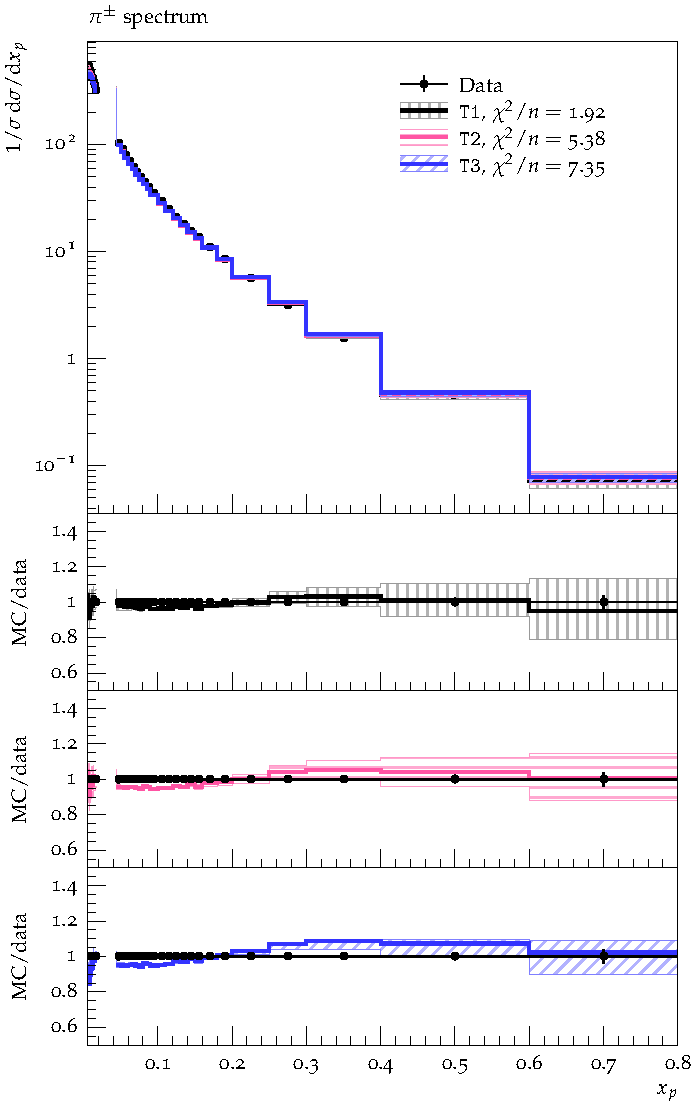
\includegraphics[width=0.47\linewidth]{New Figures/ALEPH_1996_S3486095/d25-x01-y01.pdf}
 \hfill
 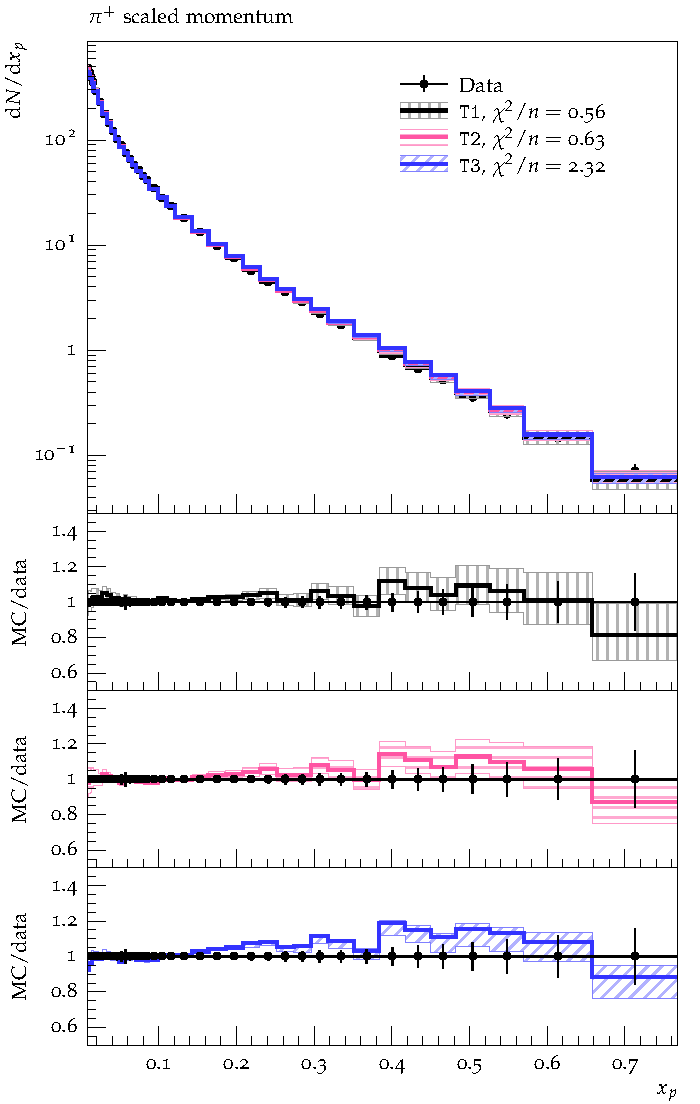
\includegraphics[width=0.47\linewidth]{New Figures/SLD_1999_S3743934/d01-x01-y02.pdf}
 \caption{$\pi^\pm$ spectrum. Data from \texttt{ALEPH$\_$1996$\_$S3486095} 
 \cite{Barate:1996fi} (left panel) and  \texttt{SLD$\_$1999$\_$S3743934} \cite{Abe:1998zs} (right panel).}
 \label{Fig.1}
\end{figure}

In Figs. \ref{Fig.1}-\ref{Fig.2}, we show $\pi^\pm$ and $\pi^0$
spectra in three different measurements and the theoretical predictions 
from the 3 tunes. We can see, except the $\pi^\pm$ spectrum in the left panel of Fig. \ref{Fig.1},
all the tunes are consistent with the experimental measurements. \\ \\

\begin{figure}[!t]
 \centering
 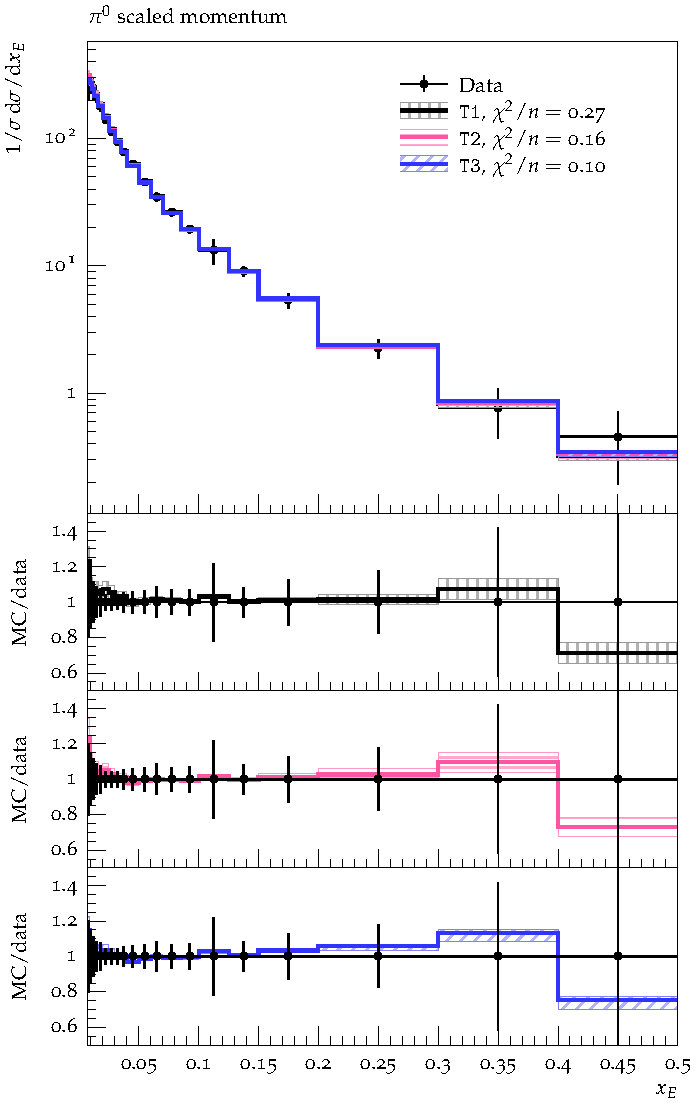
\includegraphics[width=0.47\linewidth]{New Figures/OPAL_1998_S3749908/d04-x01-y01.pdf}
 \hfill
 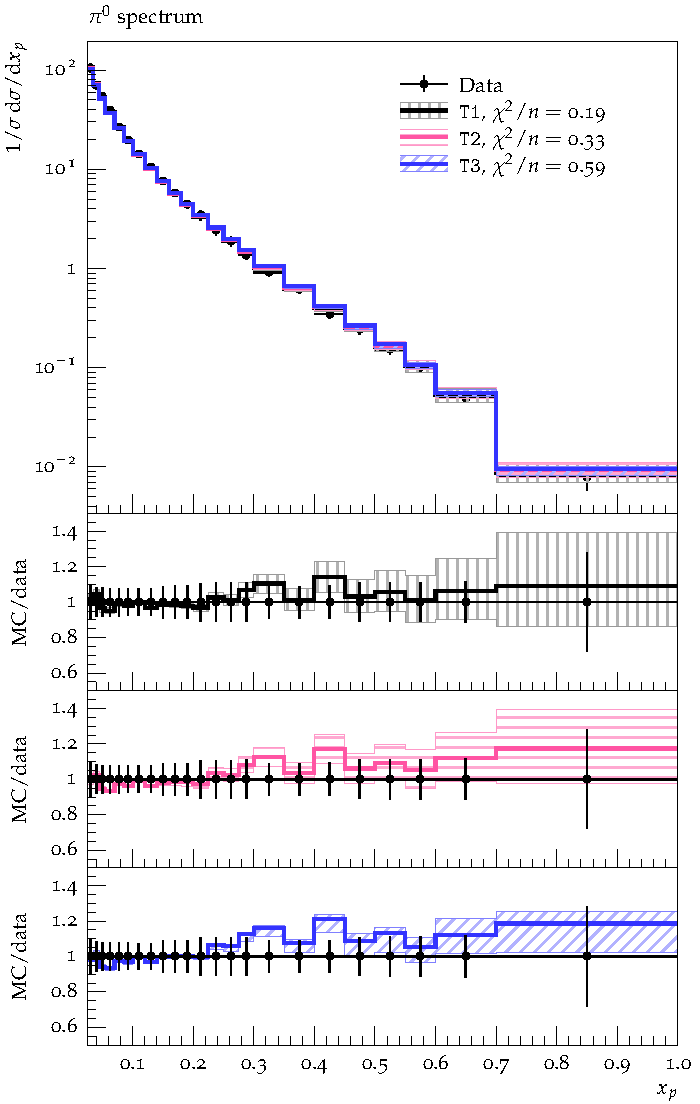
\includegraphics[width=0.47\linewidth]{New Figures/ALEPH_1996_S3486095/d29-x01-y01.pdf}
  \caption{$\pi^0$ spectrum. Date from \texttt{OPAL$\_$1998$\_$S3749908} \cite{Ackerstaff:1998ap} (left panel) and \texttt{ALEPH$\_$1996$\_$S3486095} \cite{Barate:1996fi} (Right panel).}
 \label{Fig.2}
\end{figure}


\begin{figure}[!t]
\centering
 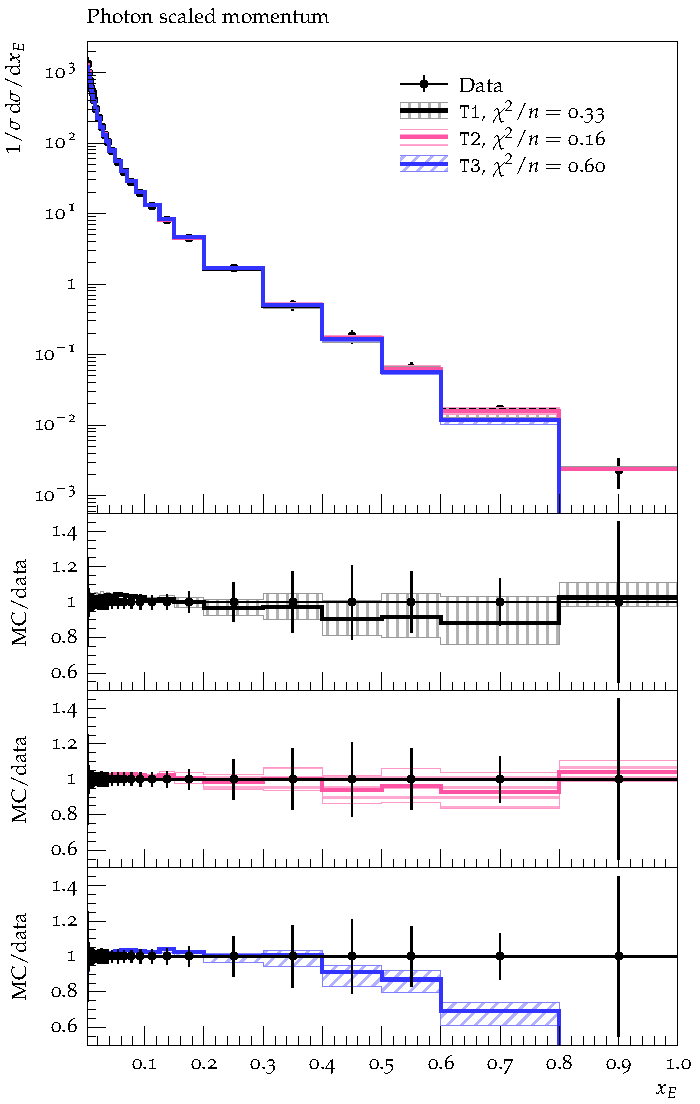
\includegraphics[width=0.47\linewidth]{New Figures/OPAL_1998_S3749908/d02-x01-y01.pdf}
 \hfill
 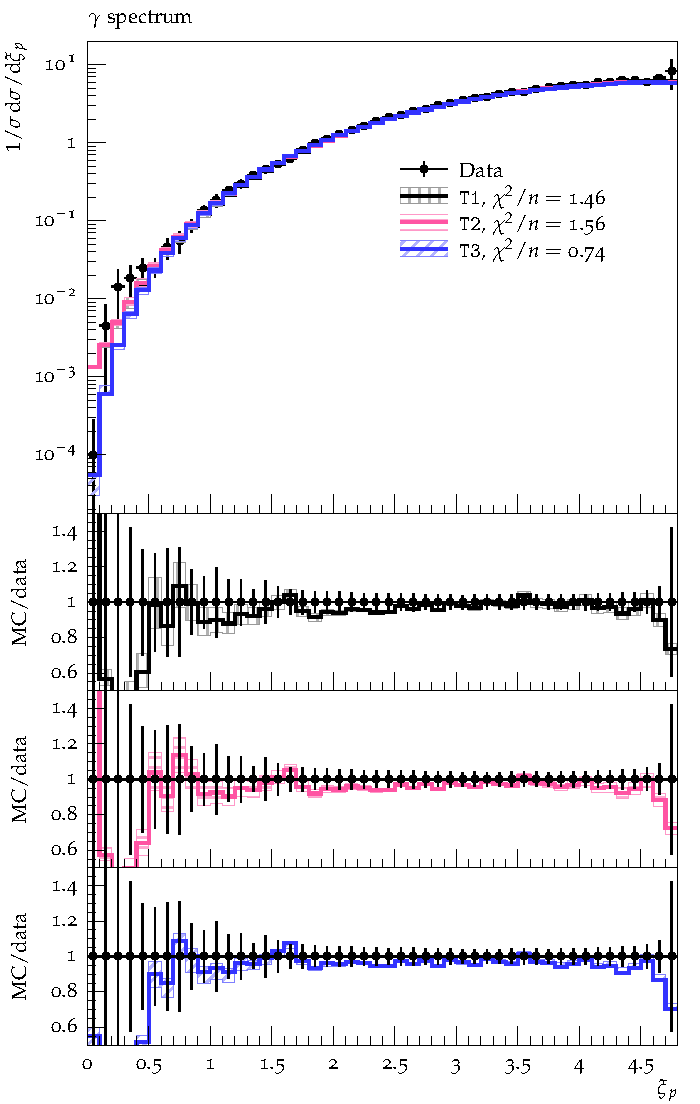
\includegraphics[width=0.47\linewidth]{New Figures/ALEPH_1996_S3486095/d28-x01-y01.pdf}
 \caption{$\pi^0$ spectrum. Data from \texttt{OPAL$\_$1998$\_$S3749908} \cite{Ackerstaff:1998ap}
 and \texttt{ALEPH$\_$1996$\_$S3486095} \cite{Barate:1996fi} (Right panel).}
 \label{Fig.3}
\end{figure}

In Figs. \ref{Fig.3}, we show the scaled
momentum distributions for photons. We can see that
the level of agreement between data and all the tunes
is perfect for $\gamma$-spectrum. \\ \\
In regard to $\eta$ spectrum, the different tunes fail to agree 
with the measurements
in certain regions of the spectrum. Nevertheless, it is
a satisfying result given that $\eta$ particles give a very small contribution
to the photon sources at LEP (and in dark matter annihilation
into jets).


\begin{figure}[!t]
 \centering
 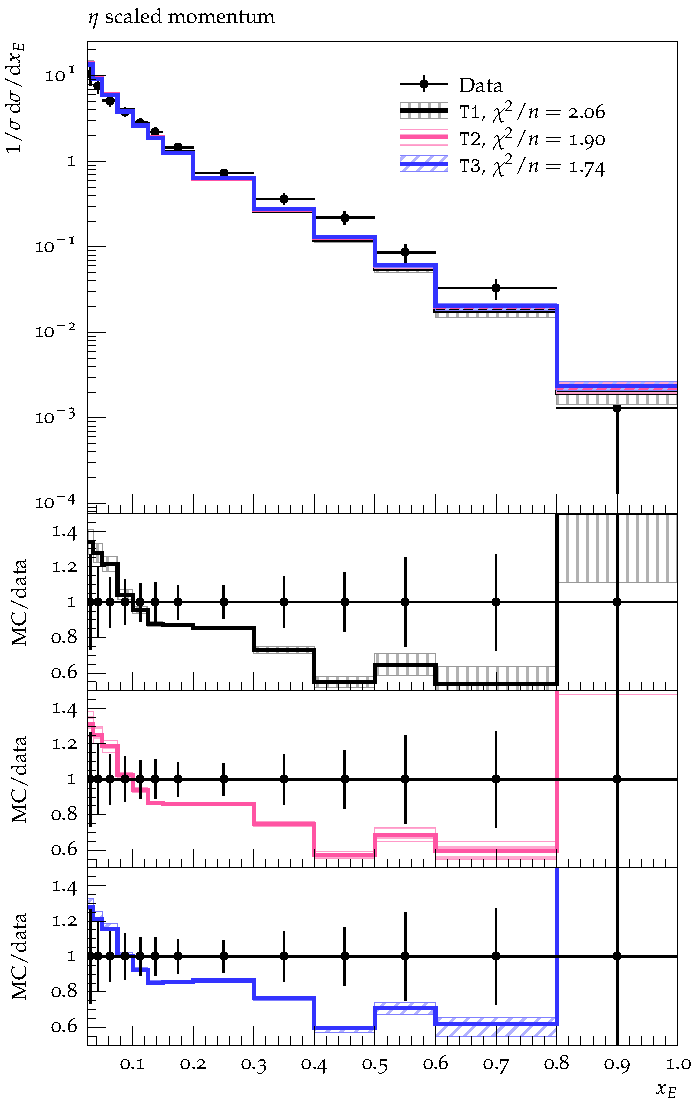
\includegraphics[width=0.47\linewidth]{New Figures/OPAL_1998_S3749908/d06-x01-y01.pdf}
 \hfill
 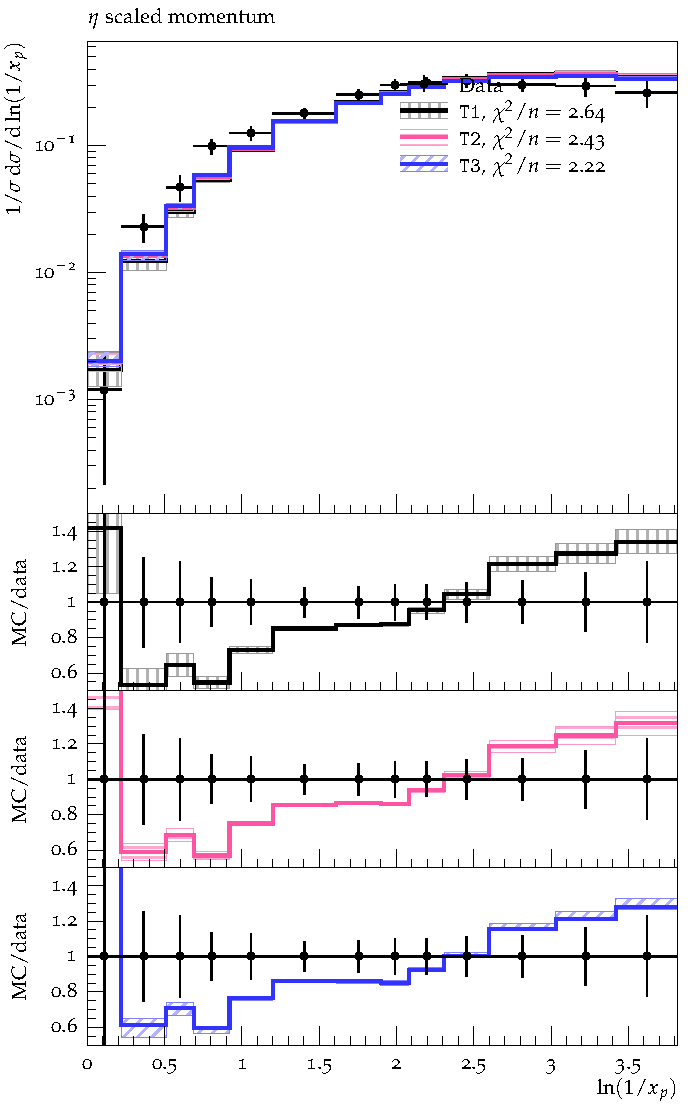
\includegraphics[width=0.47\linewidth]{New Figures/OPAL_1998_S3749908/d07-x01-y01.pdf}
  \caption{$\eta$ scaled momentum. Data from \texttt{OPAL$\_$1998$\_$S3749908} \cite{Ackerstaff:1998ap}.}
 \label{Fig.5}
\end{figure}

\clearpage
\section{Conclusions}

\appendix
\section{Observables and their weights}
 \begin{table}[!h]
  \begin{center}
   \begin{tabular}{l|l}
    \hline 
    \hline
    Observable  \hspace{3cm} &  \hspace{1cm} Associated Weight \\ \hline
    $\pi^0$ spectrum         & \hspace{3cm} $34.0$ \\ \hline
    $\pi^\pm$ spectrum       & \hspace{3cm} $70.0$ \\ \hline
    $\gamma$ spectrum        & \hspace{3cm} $70.0$ \\ \hline
    $\eta$ spectrum          & \hspace{3cm} $1.0$ \\ \hline \hline
   \end{tabular}
  \end{center}
  \caption{Identified photon and meson spectra and their weights. Data from
  \cite{Buskulic:1994ft, Barate:1996fi, Heister:2001kp, Adriani:1992hd, Akers:1994ez, Ackerstaff:1998ap, Abe:1998zs}.}
  \label{Tab1}
 \end{table}
 
 \begin{table}[tbp]
  \begin{center}
   \begin{tabular}{l|l}
    \hline 
    \hline
    Observable  \hspace{3cm}                             & \hspace{1cm} Associated Weight \\ \hline
    Mean charged multiplicity                            & \hspace{3cm} $10.0$ \\ \hline
    Mean charged multiplicity for rapidity $|Y| < 0.5$   & \hspace{3cm} $10.0$ \\ \hline
    Mean charged multiplicity for rapidity $|Y| < 1.0$   & \hspace{3cm} $10.0$ \\ \hline
    Mean charged multiplicity for rapidity $|Y| < 1.5$   & \hspace{3cm} $10.0$ \\ \hline
    Mean charged multiplicity for rapidity $|Y| < 2.0$   & \hspace{3cm} $10.0$ \\ \hline
    Mean $\pi^0$ multiplicity                            & \hspace{3cm} $10.0$ \\ \hline
    Mean $\pi^\pm$ multiplicity                          & \hspace{3cm} $10.0$ \\ \hline 
    Ratio (w.r.t $\pi^\pm$) of mean $\pi^0$ multiplicity & \hspace{3cm} $5.0$ \\ \hline
    \hline 
    \end{tabular}
  \end{center}
  \caption{Mean particle multiplicities and their weights. 
  Data from \cite{Barate:1996fi, Abreu:1996na, Ackerstaff:1998hz, Amsler:2008zzb}.}
  \label{Tab2}
 \end{table}

   \begin{table}[tbp]
  \begin{center}
   \begin{tabular}{l|l}
    \hline 
    \hline
    Observable  \hspace{3cm}                                           &  \hspace{1cm} Associated Weight \\ \hline
    Differential $3$-jet rate with Durham algorithm                    &  \hspace{3cm} $2.0$ \\ \hline
    Differential $3$-jet rate with Jade algorithm                      &  \hspace{3cm} $2.0$ \\ \hline
    Differential $4$-jet rate with Durham algorithm                    &  \hspace{3cm} $2.0$ \\ \hline
    Differential $4$-jet rate with Jade algorithm                      &  \hspace{3cm} $2.0$ \\ \hline
    Differential $5$-jet rate with Durham algorithm                    &  \hspace{3cm} $1.0$ \\ \hline
    Differential $5$-jet rate with Jade algorithm                      &  \hspace{3cm} $1.0$ \\ \hline 
    Durham jet resolution $2\to1  (E_{\text{CMS}}=91.2 \text{ GeV})$    &  \hspace{3cm} $2.0$ \\ \hline
    Durham jet resolution $3\to2  (E_{\text{CMS}}=91.2 \text{ GeV})$    &  \hspace{3cm} $2.0$ \\ \hline
    Durham jet resolution $4\to3  (E_{\text{CMS}}=91.2 \text{ GeV})$    &  \hspace{3cm} $1.0$ \\ \hline
    Durham jet resolution $5\to4  (E_{\text{CMS}}=91.2 \text{ GeV})$    &  \hspace{3cm} $1.0$ \\ \hline
    Durham jet resolution $6\to5  (E_{\text{CMS}}=91.2 \text{ GeV})$    &  \hspace{3cm} $1.0$ \\ \hline
    $2$-jet fraction $(E_{\text{CMS}}=91.2 \text{ GeV})$               &  \hspace{3cm} $2.0$ \\ \hline
    $3$-jet fraction $(E_{\text{CMS}}=91.2 \text{ GeV})$               &  \hspace{3cm} $2.0$ \\ \hline
    $4$-jet fraction $(E_{\text{CMS}}=91.2 \text{ GeV})$               &  \hspace{3cm} $2.0$ \\ \hline
    $5$-jet fraction $(E_{\text{CMS}}=91.2 \text{ GeV})$               &  \hspace{3cm} $1.0$ \\ \hline
    $\geq 6$-jet fraction $(E_{\text{CMS}}=91.2 \text{ GeV})$          &  \hspace{3cm} $1.0$ \\ \hline \hline
   \end{tabular}
  \end{center}
  \caption{Jet rates and their weights. Data from \cite{Abreu:1996na, Heister:2003aj}.}
  \label{Tab3}
 \end{table}
 
\begin{table}[tbp]
\begin{center}
\begin{tabular}{l|l}
\hline \hline 
Observable \hspace{1cm}                                        &  Associated Weight \\ \hline
In(out-)-plane $p_\bot$ in GeV w.r.t. (thrust) sphericity axes & \hspace{1cm} $2.0$ \\ \hline 
Mean out-of-plane $p_\bot$ in GeV w.r.t. thrust axis vs. $x_p$ & \hspace{1cm} $2.0$ \\ \hline
Scaled momentum $x_p=|p|/|p_\text{beam}|$                      & \hspace{1cm} $20.0$ \\ \hline
Log of scaled momentum, $\log(1/x_p)$                          & \hspace{1cm} $20.0$ \\ \hline
Energy-energy correlation, EEC                                 & \hspace{1cm} $2.0$ \\ \hline
Sphericity, $S$                                                & \hspace{1cm} $2.0$ \\ \hline
Aplanarity, $A$                                                & \hspace{1cm} $2.0$ \\ \hline
Planarity, $P$                                                 & \hspace{1cm} $2.0$ \\ \hline
$D$ parameter                                                  & \hspace{1cm} $2.0$ \\ \hline
$C$ parameter                                                  & \hspace{1cm} $2.0$ \\ \hline
1-Thrust                                                       & \hspace{1cm} $2.0$ \\ \hline
Thrust major, $M$                                              & \hspace{1cm} $2.0$ \\ \hline
Thrust minor, $m$                                              & \hspace{1cm} $2.0$\\ \hline
Oblateness, $O=M-m$                                            & \hspace{1cm} $2.0$ \\ \hline
Charged multiplicity distribution                              & \hspace{1cm} $2.0$ \\ \hline
Two-jet resolution variable, $Y3$ (charged)                    & \hspace{1cm} $2.0$ \\ \hline
Rapidity w.r.t. thrust axes, $y_T$ (charged)                   & \hspace{1cm} $2.0$ \\ \hline
Heavy jet mass $(E_{\text{CMS}} = 91.2 \text{ GeV})$           & \hspace{1cm} $2.0$ \\ \hline
Total jet broadening $(E_{\text{CMS}} = 91.2 \text{ GeV})$     & \hspace{1cm} $2.0$ \\ \hline
Wide jet broadening $(E_{\text{CMS}} = 91.2 \text{ GeV})$      & \hspace{1cm} $2.0$ \\ \hline
Jet mass difference $(E_{\text{CMS}} = 91.2 \text{ GeV})$      & \hspace{1cm} $2.0$ \\ \hline
\hline
\end{tabular}
\end{center}
\caption{Event shapes and the associated weights. Data from 
\cite{Decamp:1991uz, Barate:1996fi, Heister:2003aj, Abreu:1996na, Achard:2004sv, Abbiendi:2004qz}. }
\label{Tab4}
 \end{table}
 
 \begin{table}[tbp]
  \begin{center}
   \begin{tabular}{l | l}
\hline \hline
Observable \hspace{1cm}                                        &  Associated Weight \\ \hline
Rapidity w.r.t. sphericity axes, $y_S$                         & \hspace{1cm} $2.0$ \\ \hline
Mean $p_\perp$ in GeV vs. $x_p$                                & \hspace{1cm} $2.0$ \\ \hline
Planarity, $P$                                                 & \hspace{1cm} $2.0$ \\ \hline
Heavy hemisphere masses, $M_h^2/E_\text{vis}$                  & \hspace{1cm} $2.0$ \\ \hline
Light hemisphere masses, $M_l^2/E_\text{vis}$                  & \hspace{1cm} $2.0$ \\ \hline
Difference in hemisphere masses, $M_d^2/E_\text{vis}$          & \hspace{1cm} $2.0$ \\ \hline
Wide hemisphere broadening, $B_\text{max}$                     & \hspace{1cm} $2.0$ \\ \hline
Narrow hemisphere broadening, $B_\text{min}$                   & \hspace{1cm} $2.0$ \\ \hline
Total hemisphere broadening, $B_\text{sum}$                    & \hspace{1cm} $2.0$ \\ \hline
Difference in hemisphere broadening, $B_\text{diff}$           & \hspace{1cm} $2.0$ \\ \hline
Moments of $1 - T$ at $91$ GeV                                 & \hspace{1cm} $2.0$ \\ \hline
Moments of $M_H$ at $91$ GeV                                   & \hspace{1cm} $2.0$ \\ \hline
Moments of $C$ at $91$ GeV                                     & \hspace{1cm} $2.0$ \\ \hline
Moments of $B_\text{sum}$ at $91$ GeV                          & \hspace{1cm} $2.0$ \\ \hline
Moments of $B_\text{max}$ at $91$ GeV                          & \hspace{1cm} $2.0$ \\ \hline
Moments of $y_{23}$ at $91$ GeV                                & \hspace{1cm} $2.0$ \\ \hline
Moments of $T_\text{maj}$ at $91$ GeV                          & \hspace{1cm} $2.0$ \\ \hline
Moments of $T_\text{min}$ at $91$ GeV                          & \hspace{1cm} $2.0$ \\ \hline
Moments of $S$ at $91$ GeV                                     & \hspace{1cm} $2.0$ \\ \hline \hline    
   \end{tabular}
  \end{center}
\caption{Event shapes and the associated weights (\emph{contd}). Data from 
\cite{Decamp:1991uz, Barate:1996fi, Heister:2003aj, Abreu:1996na, Achard:2004sv, Abbiendi:2004qz}. }
\label{Tab5}
 \end{table}
 
\begin{table}[tbp]
 \begin{center}
  \begin{tabular}{ l | l }
\hline \hline
Observable \hspace{1cm}                                                  &  Associated Weight \\ \hline
Photon fragmentation function in $2$-jet events with $y_\text{cut}=0.01$ & \hspace{1cm} $1.0$ \\ \hline
Photon fragmentation function in $2$-jet events with $y_\text{cut}=0.06$ & \hspace{1cm} $1.0$ \\ \hline
Photon fragmentation function in $2$-jet events with $y_\text{cut}=0.1$  & \hspace{1cm} $1.0$ \\ \hline
Photon fragmentation function in $2$-jet events with $y_\text{cut}=0.33$ & \hspace{1cm} $1.0$ \\ \hline
Photon fragmentation function in $3$-jet events with $y_\text{cut}=0.01$ & \hspace{1cm} $1.0$ \\ \hline
Photon fragmentation function in $3$-jet events with $y_\text{cut}=0.06$ & \hspace{1cm} $1.0$ \\ \hline
Photon fragmentation function in $3$-jet events with $y_\text{cut}=0.1$  & \hspace{1cm} $1.0$ \\ \hline
Photon fragmentation function in $4$-jet events with $y_\text{cut}=0.01$ & \hspace{1cm} $1.0$ \\ \hline
\hline
  \end{tabular}
 \end{center}
 \caption{Quark-to-photon fragmentation function observables and the 
 corresponding weights. Data from \cite{Buskulic:1995au}. }
 \label{Tab6}
\end{table}


\clearpage 
\begin{thebibliography}{99}

\bibitem{Decamp:1991uz}
  D.~Decamp {\it et al.} [ALEPH Collaboration],
  %``Measurement of the charged particle multiplicity distribution in hadronic Z decays,''
  Phys.\ Lett.\ B {\bf 273} (1991) 181.
  doi:10.1016/0370-2693(91)90575-B
  %%CITATION = doi:10.1016/0370-2693(91)90575-B;%%
  
\bibitem{Buskulic:1994ft}
  D.~Buskulic {\it et al.} [ALEPH Collaboration],
  %``Inclusive pi+-, K+- and (p, anti-p) differential cross-sections at the Z resonance,''
  Z.\ Phys.\ C {\bf 66} (1995) 355.
  doi:10.1007/BF01556360
  %%CITATION = doi:10.1007/BF01556360;%%
  
\bibitem{Buskulic:1995au}
  D.~Buskulic {\it et al.} [ALEPH Collaboration],
  %``First measurement of the quark to photon fragmentation function,''
  Z.\ Phys.\ C {\bf 69} (1996) 365.
  doi:10.1007/BF02907417
  %%CITATION = doi:10.1007/BF02907417;%%
  
\bibitem{Barate:1996fi}
  R.~Barate {\it et al.} [ALEPH Collaboration],
  %``Studies of quantum chromodynamics with the ALEPH detector,''
  Phys.\ Rept.\  {\bf 294} (1998) 1.
  doi:10.1016/S0370-1573(97)00045-8
  %%CITATION = doi:10.1016/S0370-1573(97)00045-8;%%
  
\bibitem{Heister:2001kp}
  A.~Heister {\it et al.} [ALEPH Collaboration],
  %``Inclusive production of the omega and eta mesons in Z decays, and the muonic branching ratio of the omega,''
  Phys.\ Lett.\ B {\bf 528} (2002) 19
  doi:10.1016/S0370-2693(02)01220-0
  [hep-ex/0201012].
  %%CITATION = doi:10.1016/S0370-2693(02)01220-0;%%
  
\bibitem{Heister:2003aj}
  A.~Heister {\it et al.} [ALEPH Collaboration],
  %``Studies of QCD at e+ e- centre-of-mass energies between 91-GeV and 209-GeV,''
  Eur.\ Phys.\ J.\ C {\bf 35} (2004) 457.
  doi:10.1140/epjc/s2004-01891-4
  %%CITATION = doi:10.1140/epjc/s2004-01891-4;%%
  
\bibitem{Abreu:1996na}
  P.~Abreu {\it et al.} [DELPHI Collaboration],
  %``Tuning and test of fragmentation models based on identified particles and precision event shape data,''
  Z.\ Phys.\ C {\bf 73} (1996) 11.
  doi:10.1007/s002880050295
  %%CITATION = doi:10.1007/s002880050295;%%
  

\bibitem{Adriani:1992hd}
  O.~Adriani {\it et al.} [L3 Collaboration],
  %``Measurement of inclusive eta production in hadronic decays of the Z0,''
  Phys.\ Lett.\ B {\bf 286} (1992) 403.
  doi:10.1016/0370-2693(92)91795-B
  %%CITATION = doi:10.1016/0370-2693(92)91795-B;%%
  
\bibitem{Achard:2004sv}
  P.~Achard {\it et al.} [L3 Collaboration],
  %``Studies of hadronic event structure in $e^{+} e^{-}$ annihilation from 30-GeV to 209-GeV with the L3 detector,''
  Phys.\ Rept.\  {\bf 399} (2004) 71
  doi:10.1016/j.physrep.2004.07.002
  [hep-ex/0406049].
  %%CITATION = doi:10.1016/j.physrep.2004.07.002;%%
  
\bibitem{Akers:1994ez}
  R.~Akers {\it et al.} [OPAL Collaboration],
  %``Measurement of the production rates of charged hadrons in e+ e- annihilation at the Z0,''
  Z.\ Phys.\ C {\bf 63} (1994) 181.
  doi:10.1007/BF01411010
  %%CITATION = doi:10.1007/BF01411010;%%
  
  
\bibitem{Ackerstaff:1998ap}
  K.~Ackerstaff {\it et al.} [OPAL Collaboration],
  %``Photon and light meson production in hadronic Z0 decays,''
  Eur.\ Phys.\ J.\ C {\bf 5} (1998) 411
  doi:10.1007/s100520050286
  [hep-ex/9805011].
  %%CITATION = doi:10.1007/s100520050286;%%
  
\bibitem{Ackerstaff:1998hz}
  K.~Ackerstaff {\it et al.} [OPAL Collaboration],
  %``Measurements of flavor dependent fragmentation functions in Z0 --> q anti-q events,''
  Eur.\ Phys.\ J.\ C {\bf 7} (1999) 369
  doi:10.1007/s100529901067
  [hep-ex/9807004].
  %%CITATION = doi:10.1007/s100529901067;%%
  
\bibitem{Abbiendi:2004qz}
  G.~Abbiendi {\it et al.} [OPAL Collaboration],
  %``Measurement of event shape distributions and moments in e+ e- ---> hadrons at 91-GeV - 209-GeV and a determination of alpha(s),''
  Eur.\ Phys.\ J.\ C {\bf 40} (2005) 287
  doi:10.1140/epjc/s2005-02120-6
  [hep-ex/0503051].
  %%CITATION = doi:10.1140/epjc/s2005-02120-6;%%
  
\bibitem{Abe:1998zs}
  K.~Abe {\it et al.} [SLD Collaboration],
  %``Production of pi+, K+, K0, K*0, phi, p and Lambda0 in hadronic Z0 decays,''
  Phys.\ Rev.\ D {\bf 59} (1999) 052001
  doi:10.1103/PhysRevD.59.052001
  [hep-ex/9805029].
  %%CITATION = doi:10.1103/PhysRevD.59.052001;%%
  
\bibitem{Amsler:2008zzb}
  C.~Amsler {\it et al.} [Particle Data Group],
  %``Review of Particle Physics,''
  Phys.\ Lett.\ B {\bf 667} (2008) 1.
  doi:10.1016/j.physletb.2008.07.018
  %%CITATION = doi:10.1016/j.physletb.2008.07.018;%%
  
  
\bibitem{Giele:2007di}
  W.~T.~Giele, D.~A.~Kosower and P.~Z.~Skands,
  %``A simple shower and matching algorithm,''
  Phys.\ Rev.\ D {\bf 78} (2008) 014026
  doi:10.1103/PhysRevD.78.014026
  [arXiv:0707.3652 [hep-ph]].
  %%CITATION = doi:10.1103/PhysRevD.78.014026;%%
  
\bibitem{Buckley:2009bj}
  A.~Buckley, H.~Hoeth, H.~Lacker, H.~Schulz and J.~E.~von Seggern,
  %``Systematic event generator tuning for the LHC,''
  Eur.\ Phys.\ J.\ C {\bf 65} (2010) 331
  doi:10.1140/epjc/s10052-009-1196-7
  [arXiv:0907.2973 [hep-ph]].
  %%CITATION = doi:10.1140/epjc/s10052-009-1196-7;%%

  
\bibitem{Buckley:2010ar}
  A.~Buckley, J.~Butterworth, L.~Lonnblad, D.~Grellscheid, H.~Hoeth, J.~Monk, H.~Schulz and F.~Siegert,
  %``Rivet user manual,''
  Comput.\ Phys.\ Commun.\  {\bf 184} (2013) 2803
  doi:10.1016/j.cpc.2013.05.021
  [arXiv:1003.0694 [hep-ph]].
  %%CITATION = doi:10.1016/j.cpc.2013.05.021;%%
  

\end{thebibliography}

\end{document}          
